%%%%%%%%%%%%%%%%%%%%%%%%%%%%%%%%%%%%%%%%%
% Stylish Article
% LaTeX Template
% Version 1.0 (31/1/13)
%
% This template has been downloaded from:
% http://www.LaTeXTemplates.com
%
% Original author:
% Mathias Legrand (legrand.mathias@gmail.com)
%
% License:
% CC BY-NC-SA 3.0 (http://creativecommons.org/licenses/by-nc-sa/3.0/)
%
%%%%%%%%%%%%%%%%%%%%%%%%%%%%%%%%%%%%%%%%%

%----------------------------------------------------------------------------------------
%	PACKAGES AND OTHER DOCUMENT CONFIGURATIONS
%----------------------------------------------------------------------------------------

\documentclass[fleqn,10pt,ngerman]{SelfArx}
\usepackage{babel}
\selectlanguage{ngerman}

\setlength{\columnsep}{0.55cm} % Distance between the two columns of text
\setlength{\fboxrule}{0.75pt} % Width of the border around the abstract

\definecolor{color1}{RGB}{0,0,90} % Color of the article title and sections
\definecolor{color2}{RGB}{0,20,20} % Color of the boxes behind the abstract and headings

\newlength{\tocsep} 
\setlength\tocsep{1.5pc} % Sets the indentation of the sections in the table of contents
\setcounter{tocdepth}{2} % Show only three levels in the table of contents section: sections, subsections and subsubsections

\usepackage{comment}

\usepackage{fontenc}
\usepackage{inputenc}
\usepackage{url} 
\usepackage{hyperref}
\usepackage{listings}

%----------------------------------------------------------------------------------------
%	ARTICLE INFORMATION
%----------------------------------------------------------------------------------------

\JournalInfo{Software-Technik-Praktikum} % Journal information
\Archive{Sommersemester 2019} % Additional notes (e.g. copyright, DOI, review/research article)

\PaperTitle{Implementierung von REST Services zur Umsetzung der SQLcoach Anwendung} % Article title

\Authors{Max Mustermann} % Authors
\affiliation{\textit{Hochschule Kaiserslautern}} % Author affiliation
\affiliation{\textbf{Corresponding author}: Braun Daniel} % Corresponding author

\Keywords{SQL-Coach, REST, Java, Service} % Keywords - if you don't want any simply remove all the text between the curly brackets
\newcommand{\keywordname}{Keywords} % Defines the keywords heading name

%----------------------------------------------------------------------------------------
%	ABSTRACT
%----------------------------------------------------------------------------------------

\Abstract{Das Abstract ist eine maximal 200 Worte lange Zusammenfassung des Inhalts der Arbeit, so dass sich der Leser vorab ein erstes Bild vom Inhalt machen kann.}

%----------------------------------------------------------------------------------------

\begin{document}
	
	\flushbottom % Makes all text pages the same height
	
	\maketitle % Print the title and abstract box
	
	\tableofcontents % Print the contents section
	
	\thispagestyle{empty} % Removes page numbering from the first page
	
	%----------------------------------------------------------------------------------------
	%	ARTICLE CONTENTS
	%----------------------------------------------------------------------------------------
	
	\section*{Anforderungen}
	Entfernen Sie bitte diesen Abschnitt aus Ihrem fertigen Dokument und arbeiten Sie den Inhalt in den Text mit ein. 
	Ihr REST Service soll folgende User Stories abdecken.
	
	\begin{enumerate}
		
		\item Der REST-Service liefert auf Anfrage alle Szenarien mit allen Infos zu den Szenarien. 
		\item  Der REST-Service liefert auf Anfrage alle Aufgabengruppen zu einem Szenario mit allen Infos zu den Gruppen. 
		\item  Der REST-Service liefert auf Anfrage alle Aufgaben zu einer Aufgabengruppe mit allen Infos zu den Aufgaben. 
		\item  Der REST-Service erlaubt das Hinzufügen von Szenarien, Aufgabengruppen und Aufgaben.
		\item  Der REST-Service erlaubt das Ändern der Eigenschafen zu Szenarien, Aufgabengruppen und Aufgaben.
		\item  Der REST-Service erlaubt das Löschen von Szenarien, Aufgabengruppen und Aufgaben.
		\item  Der REST-Service erlaubt das Anlegen, Ändern und Löschen von Trainingsdatensätzen mit frei konfigurierbaren Datasources.
		\item  Der REST-Service erlaubt das Auslesen der Tabelleninformation aller Tabellen in einem Trainingsdatensatz (Tabelleninformation = Tabellennamen, Spaltennamen, Prim\"arschl\"ussel, Sekund\"arschl\"ussel).
		\item  Der REST-Service erlaubt das ausf\"uhrung von beliebigen 
		\textit{SELECT} Abfragen auf den Trainingsdatens\"atzen.
		\item Der Personaldatensatz von Prof. Schiefer muss mit eingebunden werden, so dass Ihr Service nach der Installation sofort einsatzbereit ist. 	
		
		
	\end{enumerate}
	
	
	Weitere Anforderungen:
	\begin{enumerate}
		
		\item Voll dokumentierter Quellcode (jede \textit{PUBLIC} Klasse und Methode hat sinnvollen JavaDoc)
		\item Guter Programmierstil (insb. Namensgebung, Funktionen, Objekte, Exceptions, Logging usw.)
		\item Zero Warnings bei SonarJava oder Intellij Code Inspection (oder Argumentation warum diese Warnung ignoriert werden kann)
		\item Exakte Einhaltung der vorgegebenen REST Schnittstellen
		\item Exakte Einhaltung der vorgegebenen maven/ docker Installation
		\item Trainingsdatens\"atze in einer von den Stammdaten unabhängiger Postgres Instanz (innerhalb von Docker). 
		\item Nachvollziehbare Branches in Ihrem GIT (Namenskonvention: SCS-[NUM]-[feature/ bugfix /doc/ refact/ test]-name) 
		
	\end{enumerate}
	
	
	\section{Einleitung} % The \section*{} command stops section numbering
	
	\addcontentsline{toc}{section}{\hspace*{-\tocsep}Einleitung} 
	
	Die Einleitung sollte ausreichenden Hintergrund für den Leser liefern, so dass er sich ohne großes Studium von Sekundärliteratur in das Thema hineindenken kann. 
	
	Es sollen hier die grundlegenden fachlichen Begriffe eingeführt werden. 
	
	Auch sollte die Motivation für die vorliegende Arbeit dargelegt werden, sowie die Zielsetzung, die man erreichen will. Weiter wird auch das Thema von eventuell verwandten Themen abgegrenzt. Hier kann auch die Literatur \cite{Harel:1987,Harel2006,Gurp99onthe} vorgestellt werden.
	
	Als Beispiel können Sie hier ein Bild des SQLCoaches einbinden (Abbildung \ref{fig:fsm1}).
	
	\begin{figure}[ht]\centering
		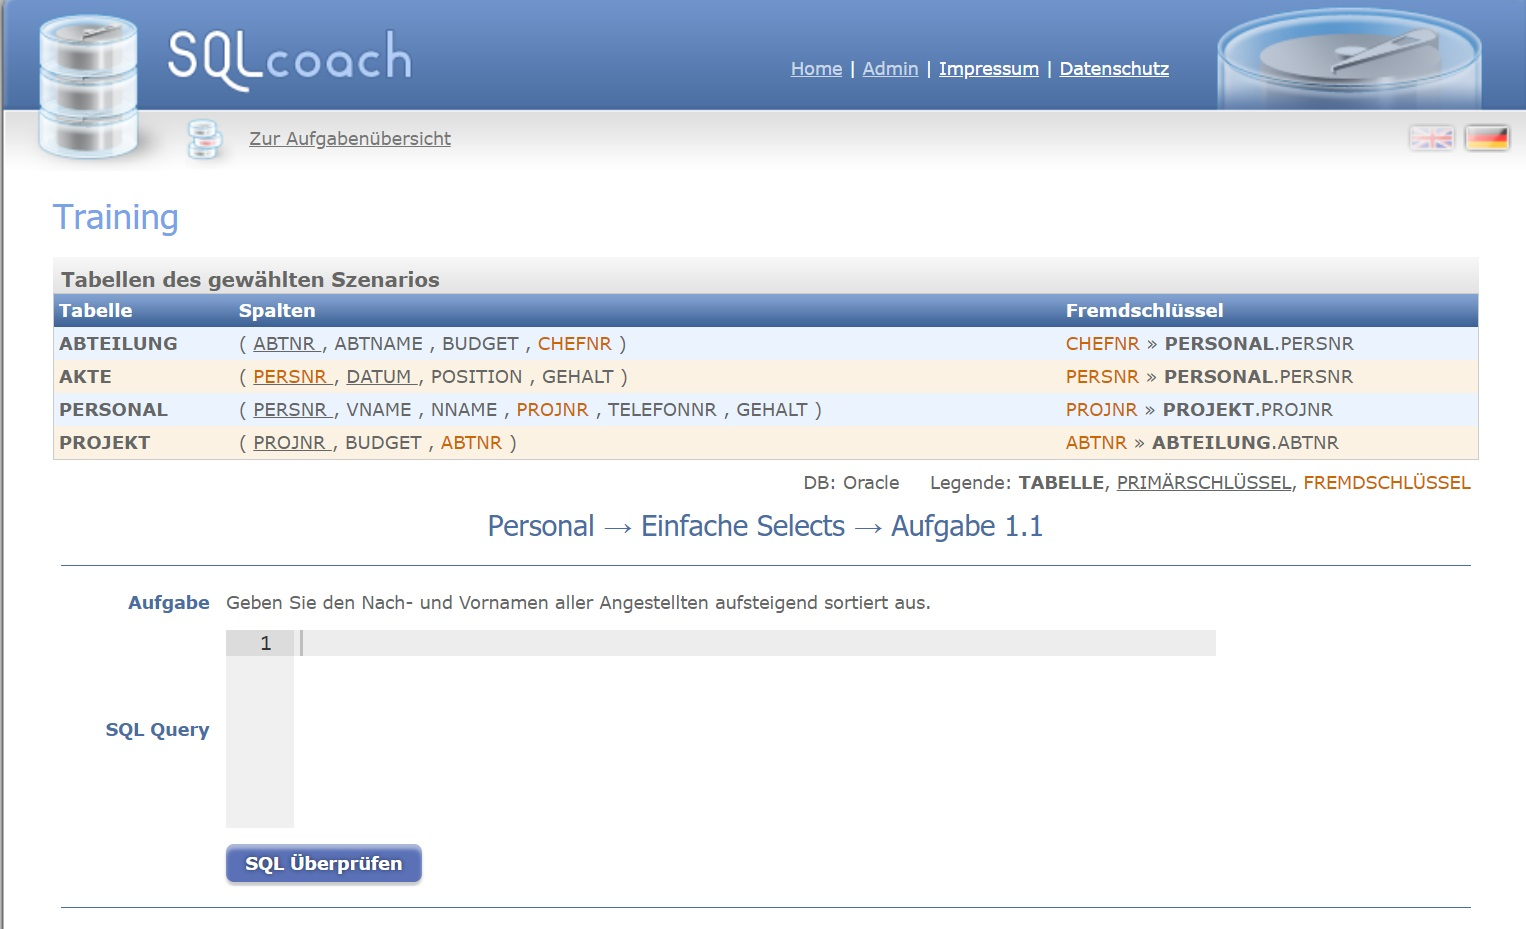
\includegraphics[width=5 cm]{Abbildungen/sqlcoach.jpg}
		\caption{Die SQLcoach Anwendung (Quelle \url{https://sqlcoach.informatik.hs-kl.de/sqlcoach/}).}
		\label{fig:fsm1}
	\end{figure}
	
	Folgende Punkte könnten hier angesprochen werden:
	\begin{itemize}[noitemsep]
		\item Sinn und Zweck der Anwendung SQLCoach.
		\item Sinn und Zweck von REST Services.
		\item Einf\"uren der wichtigen Begriffe.
		\item Welche Problemstellung wird hier bearbeitet?
	\end{itemize}
	Der SQL-Coach ist eine an der Hochschule Kaiserslautern unter der Leitunf von Dr.Prof. Schiefer entwickelte eLearning Plattform, welche sowohl das Üben als auch das Festigen von SQL-Requests auf einer Trainingsdatenbank ermöglicht. Eine Sql-Request kann beispielsweise so Elemente der Datenbank entfernen oder hinzufügen. Auf der Seite finden sich mehrere Szenarien, Aufgabengruppen und Aufgaben. 
	Eine Aufgabe beinhaltet eine Übersicht der Tabellenstrukturen aller für dieses Szenario relevanter Tabellen eine Aufgabenstellung, ein Feld in welches der Nutzer  Query/Request abtippt.(Abbildung\ref{fig:fsm2})
		\begin{figure}[ht]\centering
		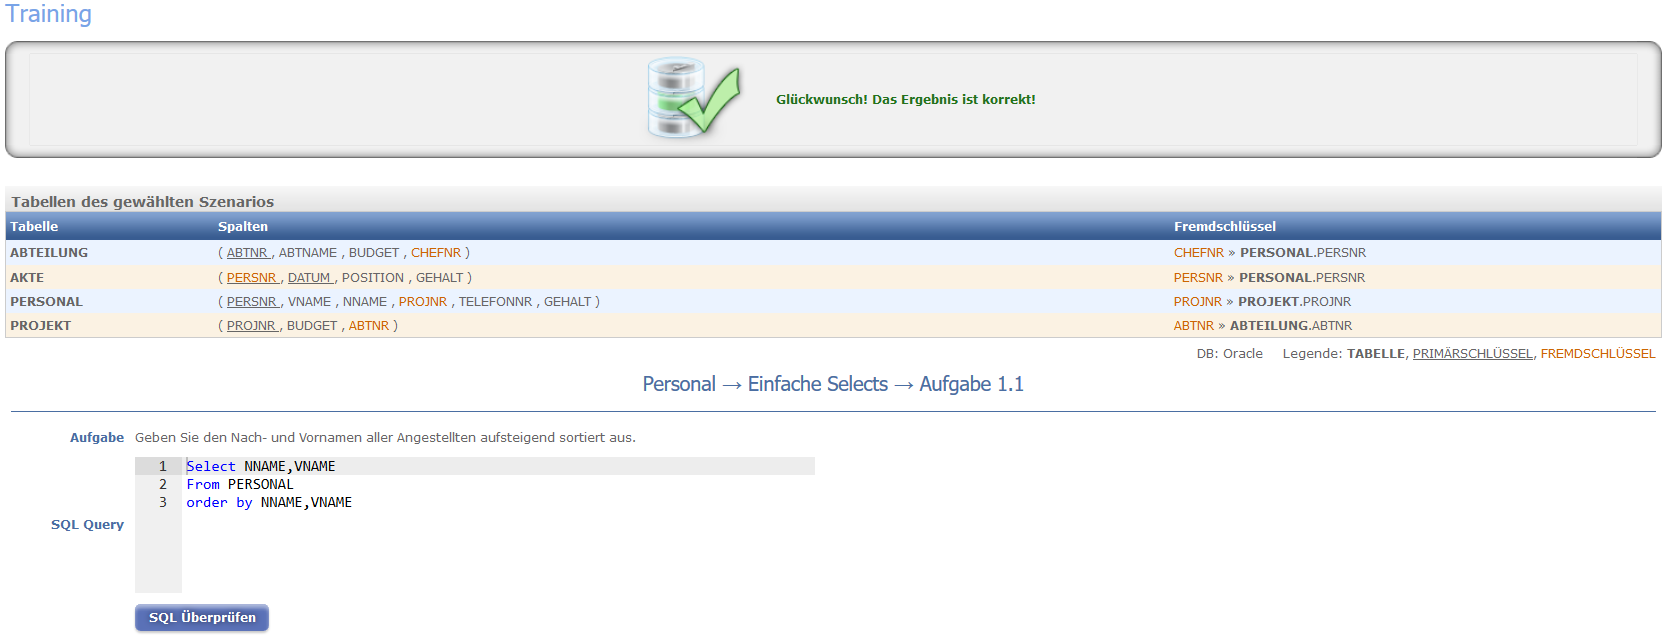
\includegraphics[width=5 cm]{Abbildungen/SQL_Coach_Aufgabe}
		\caption{Aufgabenstellung und Interface (Quelle \url{https://sqlcoach.informatik.hs-kl.de/sqlcoach/}).}
		\label{fig:fsm2}
	\end{figure}
\newline
	Ebenfalls vorhanden sind  gewünschte Ausgabe bzw. Musterlösung und die Ausgabe der vom Nutzer definierten Query aufgelistet.(Abbildung\ref{fig:fsml3})
	\begin{figure}[ht]\centering
		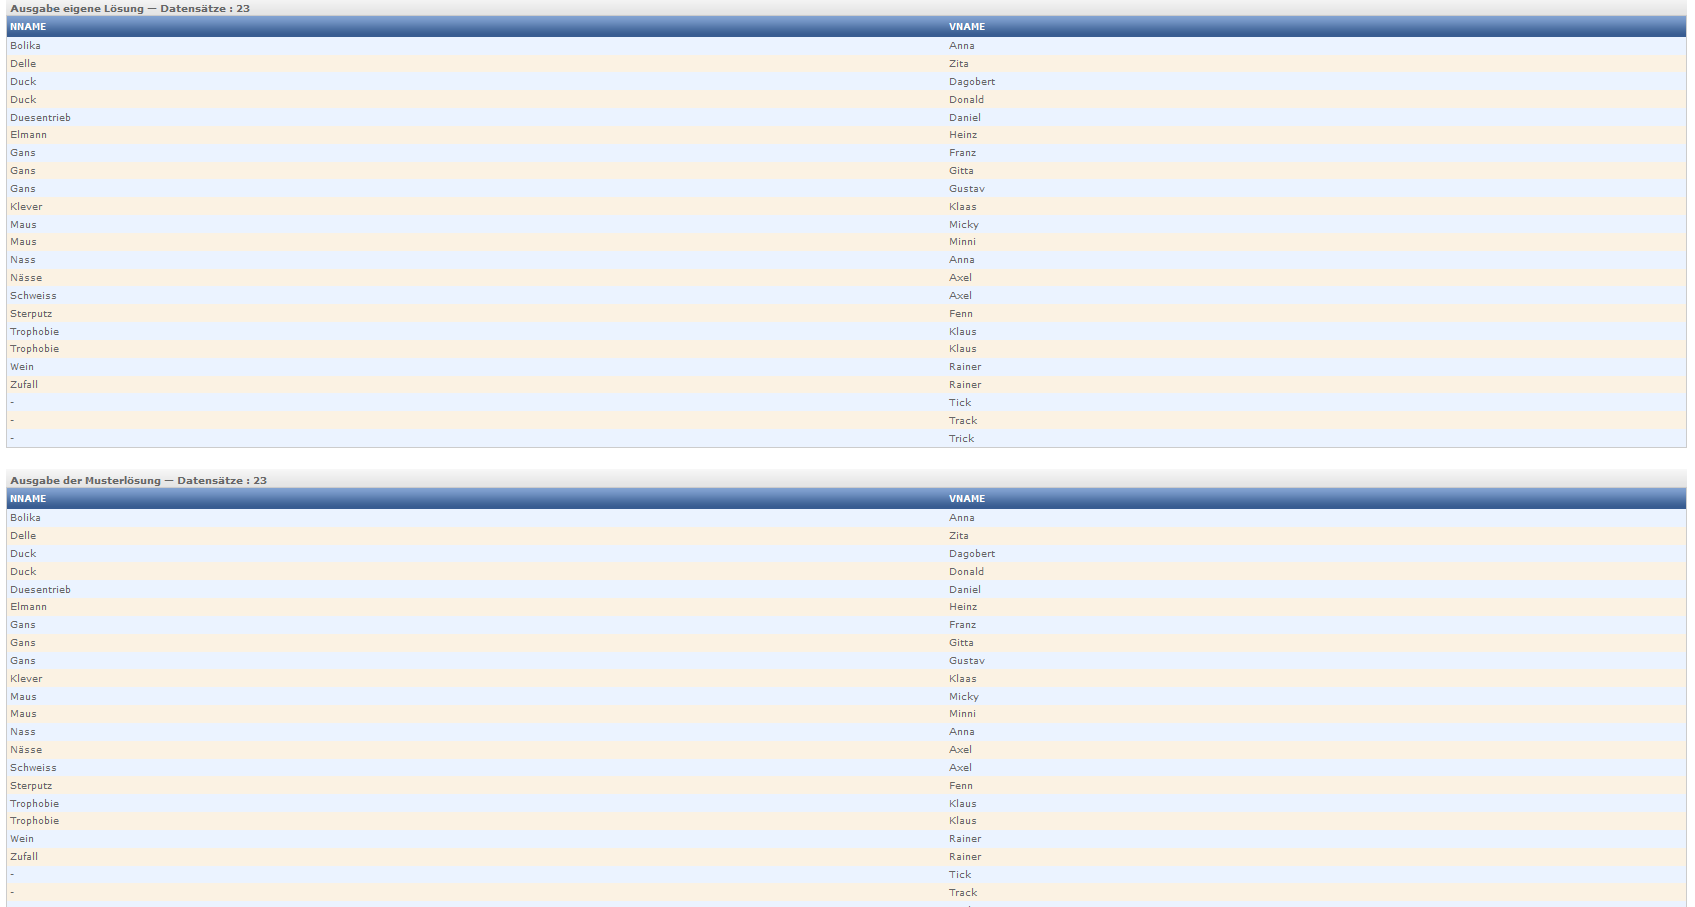
\includegraphics[width=5 cm]{Abbildungen/TabellenBild}
		\caption{Die SQLcoach Anwendung (Quelle \url{https://sqlcoach.informatik.hs-kl.de/sqlcoach/}).}
		\label{fig:fsml3}
	\end{figure}
	%------------------------------------------------
	
	
	
	
	
	
	
	%------------------------------------------------
	\newpage
	\section{Methoden und Werkzeuge}
	\label{sec:methoden}
	
	Kurze Einführung in den Abschnitt. Es wird beschrieben was jetzt kommt, d.h. welche Methoden und Werkzeuge im folgenden vorgestellt werden. 
	Es wird noch nicht darauf eingegangen was im Ganzen damit gebaut wurde. Es werden nur die Details zu den einzelnen Werkzeugen angegeben, so dass im nächsten Kapitel darauf Bezug genommen werden kann. 
	
	
	\subsection{JAX-RS und Jersey}
	JAX-RS wurde im Zuge der Tutorialreihe "REST Web Services"\footnote{\url{https://www.youtube.com/playlist?list=PLqq-6Pq4lTTZh5U8RbdXq0WaYvZBz2rbn}} als Java Programmierschnittstelle kennengelernt.
	Im Projekt wurden verschiedene Annotationen verwendet, unter anderem:\newline
	Pfad Annotationen, welche die Url der Schnittstelle definieren, der Requesttyp, welcher die Art der Anfrage definiert, sowie @Consumes und @Poduces, welche die MIME-Typ der jeweiligen akzeptierten bzw. zurückgegebenen Ressource definieren.
 
	
	\subsection{Docker}
	Docker ermöglicht die Ausführung von Anwendungen in sogenannten Container/Images, wodurch Portabilität und Kompatibilität garantiert werden. Ironischer Weise ist fehlt diese Kompatibilität bei der Installation von Docker, da  Docker auf Linux ausgelegt ist. Um Docker auf Windows laufen zu lassen wird eine Virtualbox oder Hyper-V benötigt.\footnote{Hyper-V ist Bestandteil von Microsoft Servern oder Windows 8/10 in der Pro-, Enterprise- und Education-Edition  } 
	Der Server bzw. die Datenbank läuft in einem Docker Container/Image, welcher mittels "Docker-compose build bzw.Docker-compose up" erstellt Beziehungsweise gestartet wird.
	Die hierfür notwendigen Informationen finden sich in jewils einer Dockerfile in docker\_postgres und docker\_tomcat, sowie in der Docker-compose.yml.
	Die Dockerfiles besitzen die Syntax :\newline "FROM postgres:9.6-alpine\newline 
	Copy SRC\_Path DEST\_PATH"\footnote{url{https://docs.docker.com/engine/reference/commandline/cp/}}
	Kopiert werden hier die Datenbank(en) auf das Host-system.
	
	\subsection{Maven}
	
	Zwei Sätze zur Einführung der Technologie. 
	Was wurde von dieser Technologie verwendet?
	Wie wurde von dieser Technologie verwendet?
	Welche technischen Artefakte (Dateinamen, Konfiguration, Klassen,...) sind entstanden, wie heißen diese und was machen diese. 
	
	\subsection{Postgres}
	Postgres wurde als objektrelationales Datenbankmanagementsystem (ORDBMS)"\footnote{\url{http://www.postgresql.de/index.whtml}} eingeführt und ersetzte somit Oracle SQL Developer, welcher für das Vorbildprojekt genutzt wurde. 
	Die in den sql-Dateien definierte(n) Datenbank(en) operiert mittels Postgres, weshalb auf der Datebank ausgeführte Queries auch als PostgreSQL statement formuliert sind.
	Die verwalteten Stammdaten befinden sich in der init\_database.sql Datei.  	
	
	
	\subsection{Apache Log4j}
	Zwei Sätze zur Einführung der Technologie. 
	Was wurde von dieser Technologie verwendet?
	Wie wurde von dieser Technologie verwendet?
	Welche technischen Artefakte (Dateinamen, Konfiguration, Klassen,...) sind entstanden, wie heißen diese und was machen diese. 
	
	\subsection{GIT}
	Git ist eine Filehosting-Service, der es Nutzern erlaubt hochgeladenen Code oder Code-snippets anzusehen oder diesen herunterzuladen. Auf diese weise ist es Programmierern möglich im Team an Sourcecode(-segmenten) zu arbeiten
	Zwei Sätze zur Einführung der Technologie. 
	Was wurde von dieser Technologie verwendet?
	Wie wurde von dieser Technologie verwendet?
	Welche technischen Artefakte (Dateinamen, Konfiguration, Klassen,...) sind entstanden, wie heißen diese und was machen diese. 
	
	
	
	\section{Ergebnisse}
	
	In diesem Abschnitt beschreiben Sie nun das Endergebnis Ihrer Arbeit. 
	%Endergebnisse beschreiben und Bezug auf Kap 2 nehmen
	%neutral nüchtern
	%passive nicht "ich habe oder wir haben" sondern " es wurde"
	\subsection{Architektur}
	
	Die beziehen sich hier auf die im Methodenteil vorgestellten Artefakte und beschreiben wie diese zusammengesetzt wurden. Welche Komponenten ruft welche Komponente auf? 
	
	\textbf{{Sie müssen hier auf jede der Methoden in Abschnitt} \ref{sec:methoden} Bezug nehmen.}
	
	
	\subsection{REST Schnittellen}
	Implementiert wurden, die im folgenden genauer beschriebenen Methoden, welche das Hinzufügen,Updaten und Löschen eines Szenarios, einer Aufgabengruppe oder einer Aufgabe ermöglichen. 
	Des Weiteren ist es möglich Zusatzinformationen über die implementierten Tabellen im Trainingsdatensatz zu erhalten, oder Queries auf diesen auszuführen.
	\newline
	\newline
	\noindent
	\underline{\textbf{Get all scenarios}}\newline
	\underline{http://localhost:8001/sqlcoachservice/api/v1/catalog}\newline
	\noindent Bei Aufruf der Methode getScenarios() / Aufruf der Url gibt der Restservice eine Übersicht der Szenarien in JSON-Strutur zurück. 
	Im JSON beinhaltet sind die Informationen auf welchem dataset das Szenario operiert, Rang und ID, sowie der Name des Szenarios und dessen Besitzer.
	\newline
	\newline
	\underline{\textbf{Get all groups for given scenario}}\newline
	\underline{http://localhost:8001/sqlcoachservice/api/v1/catalog}\newline\underline{/{scenarioId}}\newline
	Bei Aufruf der Methode getGroups() / Aufruf der Url gibt der Restservice eine Übersicht der Aufgabengruppen, welche Bestandteil des passenden Szenarios sind, in JSON-Strutur zurück. Durch den Pathparameter catalog/{scenarioid} ist eindeutig, dass die Aufgabengruppen des korrespondierenden Szenarios ausgegeben werden sollen. Nur die Aufgabengruppen eines Szenarios können zurückgegeben werden, weil die scenarioid  Foreign KEY ist.
	Die JSONS beinhalten die ID der Gruppe und die Id des Parent tables, sowie die Name der Aufgabengruppe.
	\newline\newline
	\underline{\textbf{Get all exercises for given group}}\newline
	\underline{http://localhost:8001/sqlcoachservice/api/v1/catalog}\newline\underline{/{scenarioId}/{groupId}}\newline
	Bei Aufruf der Methode getExercises() / Aufruf der Url gibt der Restservice eine Übersicht der Aufgaben, welche Bestandteil der passenden Aufgabengruppe sind, in JSON-Strutur zurück.
	Durch die Pathparameter ("catalog/{scenarioId}/{groupId}") sind die Foreign Keys angegeben, wodurch die Schnittstelle die gewünschten Aufgaben eindeutig identifizieren und ausgeben kann.
	Die JSONS beinhalten den Primary Key exercise ID, den foreign Key groupID, scenarioId, sowie Aufgabenbeschreibung und Aufgabenlösung.
	\newline\newline
	\underline{\textbf{Add scenario}}\newline
	\underline{http://localhost:8001/sqlcoachservice/api/v1/catalog/add}\newline
	Bei Aufruf der Methode addScenario() / / Ausführen einers ADD-Befehls (z.B. per Postman) auf dieser Url  fügt die Rest-Schnittstele, sofern ein geeignetes JSON übergeben wurde, das Szenario der Datenbank hinzu, anschließend führt er getScenario() aus und gibt somit eine Übersicht aus in der das neue Szenario vorhanden ist.\newline\newline
		\underline{\textbf{Add group for given scenario}}\newline
	\noindent\underline{http://localhost:8001/sqlcoachservice/api/v1/catalog}\newline\underline{{/scenarioId}/add}\newline
	Bei Aufruf der Methode addGroups() / Ausführen einers ADD-Befehls (z.B. per Postman) auf dieser Url fügt die Rest-Schnittstelle, sofern eine geeignete ruppe im JSON-Format übergeben wurde, die Gruppe in das durch die Pathparameter spezifizierte Szenario ein und gibt anschließend eine Übersicht der Aufgabengruppen im Szenario aus.
	\newline\newline
	
	\noindent
	\underline{\textbf{Add exercise for given group}}\newline
	\underline{http://localhost:8001/sqlcoachservice/api/v1/catalog}\newline\underline{/{scenarioId}/{grouId}/add}\newline
	Bei Aufruf der Methode addExercise() / / Ausführen einers ADD-Befehls (z.B. per Postman)  auf dieser Url fügt die Rest-Schnittstelle, sofern eine geeignete Aufgabe im JSON-Format übergeben wurde, diese in die durch die Pathparameter eindeutig bestimmte Gruppe ein und gibt anschließend eine Übersicht der Aufgaben dieser Gruppe zurück.
	\newline\newline
	
	\noindent
	\underline{\textbf{Update scenario}}\newline
	\underline{http://localhost:8001/sqlcoachservice/api/v1/catalog}\newline\underline{/{scenarioId}}\newline
	Bei Aufruf der Methode updateScenario() / Ausführen einers PUT-Befehls (z.B. per Postman) auf dieser Url ändert die Rest-Schnittstelle, sofern ein geeignetes Szenario im JSON-Format übergeben wurde, das durch den Parameter scenarioId definierte Szenario den übergebenen Werten entsprechen ab. 
	Ruft der Nutzer beispielsweise \newline http://localhost:8001/sqlcoachservice/api/v1/catalog/1 mit der Übergabe folgenden JSONS auf:\newline
	 \{      \newline
		\grqq scenarioName": "Neuer Szenarienname",\newline
		\grqq scenarioOwner": "scenarioOwner nach update ",\newline
		\grqq datasetId": 2\newline
	\}\newline
	wird der scenarioName des Szenarios mit der scenarioId 1 auf Neuer Szenarienname, scenarioOwner auf scenarioOwner nach update und die datasetId auf 2 geupdated/abgeändert.
	\newline\newline
	
	\noindent
		\underline{\textbf{Update group}}\newline
	\underline{http://localhost:8001/sqlcoachservice/api/v1/catalog}\newline\underline{/{scenarioId}/{groupId}}\newline
	Bei Aufruf der Methode updateGroup() / Ausführen einers PUT-Befehls auf dieser Url ändert die Rest-Schnittstelle, sofern eine geeignete Gruppe im JSON-Format übergeben wurde, die durch die Pathparameter definierte Gruppe den übergebenen Werten entsprechen ab. 
	\newline\newline

	\noindent
	\underline{\textbf{Update exercise}}\newline
	\underline{http://localhost:8001/sqlcoachservice/api/v1/catalog}\newline\underline{/{scenarioId}/{groupId}/scenarioId}\newline
		Bei Aufruf der Methode updateExercise() / Ausführen einers PUT-Befehls auf dieser Url ändert die Rest-Schnittstelle, sofern eine geeignete Aufgabe im JSON-Format übergeben wurde, die Werte der Aufgabe dem JSON entsprechend ab.
		\newline\newline
	
	\noindent
	
	\noindent
		\underline{\textbf{Delete scenario}}\newline
	\underline{http://localhost:8001/sqlcoachservice/api/v1/catalog/scenarioId}
	Bei Aufruf der Methode deleteScenario() / Ausführen einers DELETE-Befehls auf dieser Url wird das durch scenarioId defninierte Szenario gelöscht.
		\newline\newline
	\noindent
			\underline{\textbf{Delete group}}\newline
	\underline{http://localhost:8001/sqlcoachservice/api/v1/catalog}\newline\underline{/scenarioId/groupId}\newline
	Bei Aufruf der Methode deleteGroup() / Ausführen einers DELETE-Befehls auf dieser Url wird die durch grouId defninierte Aufgabengruppe gelöscht.
	\newline\newline
	
	\noindent
	\underline{\textbf{Delete exercise}}\newline
	\underline{http://localhost:8001/sqlcoachservice/api/v1/catalog}\newline\underline{scenarioId/groupId/exerciseId}\newline
	Bei Aufruf der Methode deleteExercise() / Ausführen einers DELETE-Befehls auf dieser Url wird die durch exerciseId defninierte Aufgabe gelöscht.
		\newline\newline
	
	\noindent
	\underline{\textbf{Get table definitions}}\newline
	\underline{http://localhost:8001/sqlcoachservice/api/v1}\newline \underline{/dataset/dataId/tables}\newline
	Das ausführen dieses Befehls gibt alle Relevanten Tabelleninformationen(Tabellen, Spalten,Primary und Foreign Keys) des Datensets mit korrespondierender dataId aus.
	\newline\newline
	
	\noindent
	\underline{\textbf{Execute query}}\newline
	\underline{http://localhost:8001/sqlcoachservice/api/v1}\newline \underline{/dataset/dataId/execute?query= \textit{query}}\newline
	Sofern hier anstelle des kursiven query eine geeignete Query steht, so wird diese auf dem durch dataId definierten Datenset ausgeführt.
	
	
	
	\subsection{Installation}
	Geben Sie hier eine Installationsanleitung. Ihre Software muss Sie wie folgt bauen und starten lassen: 
	
	\begin{lstlisting}
	git clone MYREPO
	
	mvn clean package
	
	docker-compose  build 
	
	docker-compose  up
	\end{lstlisting}
	
	
	%------------------------------------------------
	
	\section{Diskussion}
	
	In diesem Abschnitt werfen Sie einen kritischen Blick auf Ihre Arbeit:
	%
	\begin{enumerate}
		\item Haben Sie alle angeforderten User Stories umgesetzt? 
		Alle erforderlichen User-Stories wurden implementiert und wiederholt auf Funktionalität geprüft. 
		
		\item Welche Features haben sie zus\"atzlich umgesetzt?
		\item Welche positiven Eigenschaften hat Ihre Implementierung?\newline
		Vorteil der vorgestellten Implementierung von Execute Query ist, dass sie nicht nur Selects zulässt auch Delete Befehle können auf der Datenbank ausgeführt werden, weil diese aber keine Rückgabe haben erhält man eine Fehlermeldung(cause: Die Abfrage lieferte kein Ergebnis.,
		errorCode: 500,
		errorMessage: Failed to execute Query,).\newline
		Get Table Definitions gibt zwar die gewünschten Informationen in  JSON-Format zurück, dieses kann aber von der Erwartung abweichen, weil sowohl die Fremdschlüssel, als auch die Spaltennamen lediglich als Liste innerhalb des JSONS zurückgegeben werden. Vorteil dieser Implementierung ist, dass keine IF-Abfragen oder Switch-Cases den Rückgabetyp bestimmen müssen und ebenfalls keine zusätzlichen Klassen für jede im Nachhinein eingefügte Spalte erstellt werden müssen. Statt dieser Klassen ist nur die eine Klasse Table\_shemas implementiert.
		Die etwas unschöneren JSONS wurden in Kauf genommen, weil man auf diese Weise einen kürzeren Code erhält und eine einfachere Erweiterbarkeit der Datenbank.
		
		\item Welche negativen Eigenschaften hat Ihre Implementierung? 		
		\item Sind die Schnittstellen gut gelungen? Warum Sind das gute Schnittstellen? 
		\item Wie performant ist Ihre Implementierung?
		\item Welche Best Practices haben Sie eingehalten? 
		\item Wie hoch ist Ihre Test Coverage (JUnit)? 
		\item Wie ist die Code-Qualität? Berichten Sie hier über das Ergebnis der Code-Inspection (SonarJava oder IntelliJ IDEA Code-Inspection). 
		Die  IntelliJ IDEA Code-Inspection gibt mehrere zu ignorierende  Fehler aus:\newline
		 \underline{Unused declaration}{
		 	
		 }
	\end{enumerate}
	
	Dieser Abschnitt ist nicht leicht zu schreiben, aber dieser Abschnitt ist essentiell für Ihre Benotung. \textbf{Sie müssen hier das Positive herauszustellen!} Zudem sollen Sie hier auch auf Unzul\"anglichkeiten Ihrer Arbeit eingehen. Wenn Sie die Schwachstellen Ihrer Arbeit hier bel\"auchten und idealerweise Argumente finden warum das so gelöst wurde, dann hat einen sehr positiven Einfluss auf die Benotung. 
	
	
	
	\section{Zusammenfassung}
	Hier wird nochmal der Inhalt und die Ergebnisse der Arbeit kurz zusammen gefasst. Des Weiteren werden Themen und Aufgabenstellungen genannt, die es lohnt weiter zu untersuchen.
	
	%----------------------------------------------------------------------------------------
	%	REFERENCE LIST
	%----------------------------------------------------------------------------------------
	
	\bibliographystyle{unsrt}
	\bibliography{Literatur}
	
	%----------------------------------------------------------------------------------------
	
	\subsubsection*{Erklärung zur Ausarbeitung}
	Hiermit erkläre ich, Daniel Braun(880335), dass ich die vorliegende Ausarbeitung selbstständig und ohne fremde Hilfe angefertigt habe und keine anderen als in der Abhandlung angegebenen Hilfen benutzt habe; dass ich die Übernahme wörtlicher Zitate aus der Literatur sowie die Verwendung der Gedanken anderer Autoren an den entsprechenden Stellen innerhalb der Arbeit gekennzeichnet habe. Ich bin mir bewusst, dass eine falsche Erklärung rechtliche Folgen haben kann.\\ \\
	--------------------- \\
	Unterschrift
	//
	Notes:
	
	
	eth und werkz: 2 sätze was es macht/wie verwendet dann artifacts
	abgabe über olat digital gedruckte fassung ebenfalls nötig
	Begriffe einführen

	Behauptungen untermauern
	keine blümchenwörter
	Code zählt nicht als text
	keine website sondern ne webbasierte anwendug wurde erstellt
	
ziel: moderne Technologien (wie jax rs)
visuell ansprechend
Zusammenfassugn 200 wörter zusammenfassug der arbeit
Einleitung:wann wurde sql coach ersstellt 2007 unter leitung prof. schiefer
ist veraltet es wird bsp das  mvc Framework apache struts
	keine website sondern ne webbasierte anwendug wurde erstellt
	http standartmethoden, get post put delete
	
	Jax rs ist eine java api spezifikation," welche die Rest architektur bereitstellt und seit Version 6 offiziell bestandteil der Java EE Pakete ist."
	Jersey(referenz) implementiert die Jax-RS Schnittstelle.
	
	dir in latex mit \\dirtree{%
		
		.1SQL-coa...
		.2.....
		.3etc
	}
	Docker: Anwedunug werden isoliert und laufen in container
	werden aud f anderen Rechenrn beeitgestellt
	referenz zu docker
	
	werkzeuge:	Scöpfer und baujahr 
	
	dockerfile:Dieses Dockerfile spezifiziert den  PHP Webserver Apache 7.2.siehe section\ref{sec:php}
	szenarien gezielt eine topic vermittelnd ding lehrend.
	"Die Informationen zu Szenarien--....datensätzen datasources werden in der sogenannten catalog datenbank abgelegt, Zusätzlich gibt es den begriff der trainingsdatenbank welche  datensätze für die ausführnung der sql abfragen enthalten
	
	{[(docker compose eigene db 8004:80)]}
	    am ende der einleitung: was in wlechem kapitel ist
	    2:in diesem abschnitt werde die genutzten Methoden und Werkzeuge erklärt.sql coach läuft af max db wurde in postgres überführt. 
	    
	    2:
rest ist ein architekturstil, der die kommunikation zwischen Rechnern vereinfachen soll.
Er wird überwiegen für Webservices im Client-Server-Modell verwendet.
.Die implementierung von servern cient kann unabhängig erfolgen. Es gibt sechs Prinzipien die erfüllt werden müssen, aber die Implementierung ist nicht festgelegt:-...



JAxrs:JAX-RS ist eine Spezifikation einer API von Java, die es ermäglicht REST zu verwenden. Glassfish Jersey ist eine Open-Source Implementierung von JAX-RS, dief für dieses Projekt genutzt wird....

catressource: Die klasse definiert die Rest-endpunkte für die verwaltung..


Tomcat apache tomcat ist oensource.webserver...Er erlaubt es in java geschriebene web anwendungen...

meth und werkzeuge ebenfalls tomcat?

docker: beggel approved:	
 software die es ermöglicht ganze programme in containern zu kapseln. In einem container sollte das programm und alle Abhängigkeiten davon vorhanden sein.Programm ist systemunabhängig und läuft auf jedem Rechner mit Linux oder windows betriebssystem. Gemäß der Docker-Design-Vorgaben soll pro container nur ein prozess laufen, weshalb die sql coach anwendung auf einem Tomcat-Docker-Container und zwei Datenbank-DockerCoontainer umgesetzt wurde.
 
 
 
 Die Docker-Compose-Datei i docker-compose.yml (reference ocker compopse page) spezifiziert die drei Images für die  oben erwähnten Container. In dieser Datei werden auch die Ports, die Abhängigkeiten und die Pverwendeten psswörter spezifiziert. (welche datei macht was?)
Der Container für die Katalogdatenbank wird auf Basis des Images postgres:9.6-alpine erstellt. Der SQL-Coachservice wird mit docker/tomcate/dockrfile erstellt und mit Hilfe der  \textit{init\database.sql} initialisiert. 

Zunächst wird die Katalogdatenbank mit der socker/posgres/dockerfile erstellt.

apache maven:
Maven ist ein Build-Management-Tool. Maven beschreibt die Abhängigkeiten und verwaltet den Build-Prozess der Anwendung .((macht dependancy management)organisiert build prozess).
Die pom.xml //(passt wsl nicht:Datei beschreibt welche Anwendungen erstellt werden und werden nach der Erstellung in den target Ordner eingefügt.) 

Die folgenden Dependencies werden über die pom.xml spezifiziert:

Jersey
jackson
log4j
hikari
jaxb

....
POstgres:

GIT:welches repository verwendet man


Abstract:Die Anwendung SQLcoach veraltetes framework apache struts
Architektur:nicht auf paketebene runter gehen
laex links: kasten unteredrücken
\usepackage[hidelinks]{hyperref}
\end{document}